\documentclass[a4paper,12pt,openany]{article}
\usepackage{fancyhdr}
\usepackage[T1]{fontenc}
\usepackage[margin=1.8cm]{geometry}
\usepackage[applemac]{inputenc}
\usepackage{lmodern}
\usepackage{enumitem}
\usepackage{microtype}
\usepackage{hyperref}
\usepackage{enumitem}
\usepackage{dsfont}
\usepackage{amsmath,amssymb,amsthm}
\usepackage{mathenv}
\usepackage{amsthm}
\usepackage{graphicx}
\usepackage[all]{xy}
\usepackage{lipsum}       % for sample text
\usepackage{changepage}
\theoremstyle{plain}
\newtheorem{thm}{Theorem}
\newtheorem*{thm*}{Th\'eor\`eme}
\newtheorem{prop}[thm]{Proposition}
\newtheorem{cor}[thm]{Corollary}
\newtheorem{lem}[thm]{Lemma}
\newtheorem{propr}[thm]{Propri\'et\'e}
\theoremstyle{definition}
\newtheorem{deff}[thm]{Definition}
\newtheorem{rqq}[thm]{Remark}
\newtheorem{ex}[thm]{Exercice}
\newcommand{\e}{\mathrm{e}}
\newcommand{\prodscal}[2]{\left\langle#1,#2\right\rangle}
\newcommand{\devp}[3]{\frac{\partial^{#1} #2}{\partial {#3}^{#1}}}
\newcommand{\w}{\omega}
\newcommand{\dd}{\mathrm{d}}
\newcommand{\x}{\times}
\newcommand{\ra}{\rightarrow}
\newcommand{\pa}{\partial}
\newcommand{\vol}{\operatorname{vol}}
\newcommand{\dive}{\operatorname{div}}
\newcommand{\T}{\mathbf{T}}
\newcommand{\R}{\mathbf{R}}
\newcommand{\Z}{\mathbf{Z}}
\newcommand{\N}{\mathbf{N}}
\newcommand{\C}{\mathbf{C}}
\newcommand{\F}{\mathcal{F}}
\newcommand{\Tcal}{\mathcal{T}}
\newcommand{\Rcal}{\mathcal{R}}
\newcommand{\Zcal}{\mathcal{Z}}
\newcommand{\Ncal}{\mathcal{N}}
\newcommand{\Ccal}{\mathcal{C}}
\newcommand{\Acal}{\mathcal{A}}
\newcommand{\Fcal}{\mathcal{F}}
\newcommand{\Pcal}{\mathcal{P}}
\newcommand{\Scal}{\mathcal{S}}
\newcommand{\Homeo}{\mathrm{Homeo}}
\renewcommand{\x}{\mathbf{x}}
\newcommand{\Matn}{\mathrm{Mat}_{n \times n}}
\DeclareMathOperator{\tr}{tr}
\newcommand{\id}{\mathrm{id}}
\newcommand{\htop}{h_\mathrm{top}}


\title{\textsc{Syst \`emes dynamiques} \\ Feuille d'exercices 8}
\date{}
\author{}

\begin{document}

{\noindent \'Ecole Normale Sup\'erieure  \hfill  \texttt{chaubet@dma.ens.fr} } \\
{2020/2021 \hfill}

{\let\newpage\relax\maketitle}
\maketitle

\noindent {\large \textbf{Exercice 2} \textit{Th\'eor \`emes d'extension : rappels}} \vspace{1.5mm} 
\begin{enumerate}
\item Soit $E$ un ensemble et $\Acal \subset \Pcal(E)$ une alg\`ebre de Boole, c'est-\`a-dire que $\emptyset \neq \Acal$ et pour tous $A,B \in \Acal$ on a
$$A \setminus B \in \Acal \quad \text{ et } \quad A \cup B \in \Acal.$$

%\vspace{0.2cm}
Soit $\mu : \Acal \to [0, \infty]$ une mesure sur $\Acal$, c'est-\`a-dire que $\mu(\emptyset) = 0$ et pour toute s\'equence $(E_i) \in \Acal^\N$ telle $E_i \cap E_j = \emptyset$ si $i \neq j$ on a 
$$
\bigcup_{i \in \N} E_i \in \Acal \quad \implies \quad \sum_{i\in \N} \mu(E_j) = \mu \left(\bigcup_{i \in \N} E_i\right).
$$
\begin{thm*}[Carath\'eodory]
Il existe une mesure $\mu^* : \sigma(\Acal) \to [0, \infty]$ qui \'etend $\mu$. Si $\mu$ est $\sigma$-finie, alors $\mu^*$ est unique.
\end{thm*}

\item Le th\'eor\`eme est le suivant.
\begin{thm*}[Classe monotone]
On suppose que $\Pi$ est un $\pi$-syst\`eme (i.e. un sous-ensemble de parties de $E$ stable par intersections finies). Alors
$$
\bigcap_\Ccal \Ccal = \sigma(\Pi),
$$
o\`u l'intersection porte sur l'ensemble des classes monotones $\Ccal$ telles que $\Pi \subset \Ccal$.
\end{thm*}
\end{enumerate}
\vspace{0.6cm}

\noindent {\large \textbf{Exercice 3.} \textit{Tribu produit}} \vspace{1.5mm} 


\begin{enumerate}
\item $\Fcal^{\otimes \N}$ est par d\'efinition la tribu engendr\'ee par les cylindres.
\item Si $A = A_1 \cup \cdots \cup A_n$ avec $A_i \in \Scal$ et $A_i \cap A_j = \emptyset$ si $i \neq j$, on pose
$$
\mu(A) = \sum_{i=1}^n \mu(A_i).
$$
%\pau
Si $A$ s'\'ecrit aussi $A_1' \cup \cdots \cup A_m'$, alors
$$
\sum_{j=1}^m \mu(A_i') = \sum_{i,j} \mu(A_i' \cap A_j) = \sum_{j=1}^n \mu(A_j),
$$
donc $\mu(A)$ ne d\'epend pas de la d\'ecomposition choisie.

%\pau
\vspace{0.2cm}
On v\'erifie alors facilement que $\mu$ d\'efinit bien une mesure sur $\Scal.$

\item On se donne $P$ une mesure de probabilit\'e sur $A$ et on note $\Scal$ l'ensemble des cylindres. On d\'efinit $\mu : \Scal \to [0, +\infty]$ par $\mu(\emptyset) = 0$ et
\begin{equation}\label{eq:prod}
\mu\left(C_{n,\mathbf{A}}\right) = \prod_{j=1}^p P(A_j), \quad \mathbf{A} = (A_1, \dots, A_p) \in \mathcal{F}^p.
\end{equation}
On se donne des cylindres $S^n = S^n_0 \times S^n_1 \times \cdots \in \Scal$, ($n \in \N$) tels que $X= \bigcup_n S^n$ ; pour tout $k \in \N$ on consid \`ere
$
H_k : A^{k+1} \to [0,1]
$
d\'efinie par
$$
H_k(x_0, \dots, x_k) = \sum_{n \geq 0} \left( \prod_{j > k} P(S^n_j)\right)\left(\prod_{i=0}^k 1_{S^n_i}(x_i)\right).
$$
\begin{enumerate}
\item On a
$$
\begin{aligned}
\int_A H_{k+1}(x_0, \dots, &x_k, x) \dd P(x) \\
&= \int_A  \sum_{n \geq 0} \left( \prod_{j > k+1} P(S^n_j)\right)\left(\prod_{i=0}^{k} 1_{S^n_i}(x_i)\right) 1_{S^n_{k+1}}(x) \dd P(x) \\
&= \sum_{n \geq 0} \left( \prod_{j > k+1} P(S^n_j)\right)\left(\prod_{i=0}^{k} 1_{S^n_i}(x_i)\right) P(S^n_{k+1}) \\
&= H_k(x_0, \dots, x_k).
\end{aligned}
$$
\item On a 
$$
\int_A H_0(x) \dd P(x) = \int_A \sum_{n \geq 0} \left( \prod_{j >0} P(S^n_j)\right)1_{S^n_0}(x)\dd P(x) = \sum_n \mu(S^n) < 1.
$$
%\pau
Ainsi il existe $x_0 \in A$ tel que $H_0(x_0) < 1.$ On suppose construits $x_0, \dots, x_k \in A$ tels que $H_k(x_0, \dots, x_k) < 1.$
%\pau
\vspace{0.2cm}
Alors par (a) on a
$$
\int_A H_{k+1}(x_0, \dots, x_k, x) \dd P(x) = H_k(x_0, \dots, x_k) < 1.
$$
%\pau
Ainsi il existe $x_{k+1} \in A$ tel que $H_{k+1}(x_0, \dots, x_{k+1}) < 1$.
\item Par la question \textbf{2.}, l'application $\mu$ s'\'etend uniquement en une mesure additive sur l'ensemble des unions de cylindres. On veut appliquer le th\'eor\`eme de Carath\'edory. Pour cela, on aimerait montrer que $\mu$ est $\sigma$-additive (il suffit de le montrer sur les cylindres). Soit $(S^n)$ une suite de cylindres deux-\`a-deux disjoints telle que $X = \cup_n S^n$. On suppose par l'absurde que $\sum_n \mu(S^n) < 1.$ Par (b), il existe une suite $\mathbf{x} = (x_n)$ telle que $H_k(x_0, \dots, x_k) < 1$ pour tout $k$. Soit $m \in \N$ tel que $x \in S^m$, et $i_m \in \N$ tel que $S^m_i = A$ pour tout $j > i_m.$ Alors on a
$$
\left(\prod_{j > i_m}P(S^m_i)\right) \left(\prod_{i=0}^{i_m} 1_{S^m_i}(x_i)\right) = 1,
$$
%\pau
et donc 
$$
H_{i_m}(x_0, \dots x_{i_m}) \geqslant \left(\prod_{j > i_m}P(S^m_i)\right) \left(\prod_{i=0}^{i_m} 1_{S^m_i}(x_i)\right) = 1,
$$
%\pau
ce qui est absurde.

Montrons maintenant que $\mu$ est invariante par le d\'ecalage $\sigma : X \to X$. d\'efini par
$$
\sigma : (x_n) \mapsto (x_{n+1}).
$$ 
%\pau
Soit $S = S_0 \times S_1 \times \cdots$ un cylindre. Alors
$$\sigma^{-1}(S) = A \times S_0 \times S_1 \times \cdots,$$
%\pau
et donc $\mu(\sigma^{-1}(S)) = \mu(S).$ Cette \'egalit\'e est donc aussi vraie pour tout $S \in \Fcal^{\otimes \N}.$

\end{enumerate}

\item La seule difficult\'e est la $\sigma$-additivit\'e. On se donne une suite de cylindres $(S^n)$ comme pr\'ec\'edemment.
%\pau


On pose 
$$
F_N = \complement \left(\bigcup_{n \leqslant N}�S^n\right).
$$
%\pau
Alors $F_N$ est une suite d\'ecroissante de compacts, telle que l'intersection $\bigcap_N F_N$ est vide. 
%\pau


Ceci implique que $F_N = \emptyset$ si $N$ est assez grand, et donc $\cup_{n \geqslant N} S^n = A^{\N}$. En particulier $\mu(\cup_{n \leqslant N} S^n) = 1.$


\item $P_M$ est additive car si $\mathbf{w} = (w_0, \dots, w_p) \in A^{p+1}$ on a d'un c�t\'e
$$
\mu\left(\bigcup_{i=1}^m C_{n, i\mathbf{w}}\right) = \mu(C_{n+1, \mathbf{w}}) = v_{w_0} \prod_{j=0}^{p-1} m_{w_j, w_{j+1}},
$$
%\pau
et de l'autre, puisque $v = Mv$,
$$
\sum_{i=1}^m \mu(C_{n,i\mathbf{w}}) = \sum_{i=1}^m v_i m_{i, w_0}\prod_{j=0}^{p-1}m_{w_j, w_{j+1}} = \left(\prod_{j=0}^{p-1}m_{w_j, w_{j+1}}\right) \underset{v_{w_0}}{\underbrace{\sum_{i=1}^m v_i m_{i, w_0}}}.
$$
L'existence et l'unicit\'e de $P_M$ sont alors claires par le m\^eme raisonnement qu'aux questions pr\'ec\'edentes. Il suffit donc de montrer que $P_M$ est une mesure de probabilit\'es invariante par le d\'ecalage.
%\pau

C'est une mesure de probabilit\'es :
$$
P_M(X) = \sum_{w \in A} \mu(C_{0, w}) = \sum_{i=1}^m v_i = 1.
$$
%\pau
De plus $P_M$ est $\sigma$-invariante car $\sigma^{-1}(C_{n,\mathbf{w}}) = C_{n+1, \mathbf{w}}.$


\item On se donne un mot $\mathbf{w} = (w_0, \dots, w_{p})$. Alors
$$
P^{\otimes \N}(C_{n,\mathbf{w}}) = \prod_{j=0}^p P(\{w_j\}) = P(\{w_0\}) \prod_{j=0}^{p-1} M(P)_{w_j, w_{j+1}},
$$
%\pau
ce qui conclut car si $v = (P(\{1\}), \cdots, P(\{m\}))$ on a  $vM(P) = v.$



\item Soit $\mathbf{w} = (w_0, \dots, w_p) \in A^{p+1}$. Alors $x \in H(C_{n, \mathbf{w}})$ si et seulement si
$$
\forall j = 0, \dots, p,  \quad m^{n+j}x \in \left[\frac{w_j-1}{m}, \frac{w_j}{m}\right[ \mod \Z.
$$
%\pau
Par suite on a, puisque $x \mapsto m^nx$ pr\'eserve la mesure de Lebesgue sur $\R / \Z$,
$$
\mathrm{Leb}(H(C_{n, \mathbf{w}})) = \mathrm{Leb}\left(\bigcap_{j=0}^p \left\{x \in \R/\Z,~m^jx \in I_j\right\} \right) = \frac{1}{m^{p+1}}
$$
%\pau
\begin{figure}
\begin{center}
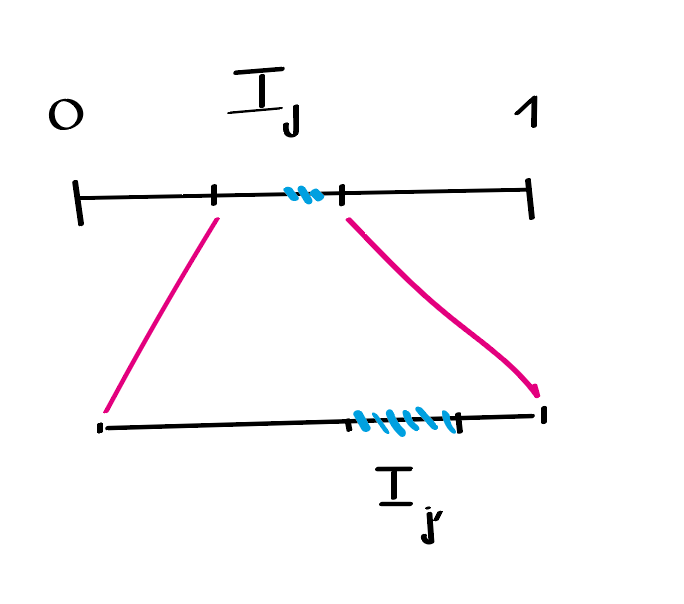
\includegraphics[scale = 0.5]{interval.png}
\end{center}
\end{figure}
%\pau
Or
$$
\mu_m^{\otimes \N}(C_{n, \mathbf{w}}) = \prod_{j=0}^p P(\{w_j\}) = \frac{1}{m^{p+1}}.
$$


\item  L'ensemble $\complement Z$ des points $m$-adiques est d\'enombrable, notons le $\{y_k,~�k\in\N\}$. On a alors
$$
\mathrm{Leb}\left(\complement Z\right) = \sum_{k} \mu(\{y_k\}) = 0.
$$

\item Si $\mathbf{x} \in H^{-1}(Z)$, alors $\mathbf{x}$ ne stationne pas \`a $1$ ni $m$ \`a partir d'un certain rang.

%\pau

On a
$$
\begin{aligned}
H(\sigma(\mathbf{x})) &= \sum_{k=1}^\infty \frac{x_{k+1} - 1}{m^k}�\mod \Z \\
%\pau
&= m H(\mathbf{x}) \mod \Z.
\end{aligned}
$$
%\pau
Il est clair que $x \in \R/\Z$ qui n'est pas $m$-adique admet exactement un ant\'ec\'edent par $H$, en regardant les nombres $x_k \in \{1, \dots, m\}$ ($k \in \N_{\geqslant 1}$) tels que
$$
x_k - 1 = \lfloor m^{k} x \rfloor \mod m,
$$
qui ne stationnent jamais \`a $1$ ou $m$.
\end{enumerate}


\end{document}

\noindent {\large \textbf{Exercice 8.} \textit{Flots hamiltoniens}} \vspace{1.5mm} 

\noindent Soit $H : \R^{2n} \to \R$ une fonction lisse. Le champ hamiltonien $X$ associ\'e  \`a $H$ est le champ de vecteurs sur $\R^{2n}$ d\'efini par

$$ X(x, \xi) = J \cdot \nabla H (x,\xi), \quad (x,\xi) \in \R^{2n},$$
o \`u $J = \begin{pmatrix} 0 & I_n \\ -I_n & 0 \end{pmatrix}$. On suppose qu'il existe une application lisse $A : \R^n \to S_n(\R)$ telle que $A(x)$ est d\'efinie positive pour tout $x$ et
$$
H(x,\xi) = \frac{1}{2} \bigl\langle A(x)\xi, \xi \bigr\rangle, \quad (x,\xi) \in \R^{2n}.
$$


\vspace{0.6cm}




\end{document}
 
